\chapter{Verification \& Validation}
\emph{Validation} is the task that verifies if the software system is the right one according to its effectiveness, external, i.e.,\@  versus user, and reliability. \emph{Verification} is the task that verifies if the software system is right according to its efficiency, internal, i.e.,\@ correctness of vertical transformations, and correctness.

\paragraph{Scenario 1}
\begin{itemize}
\item Stakeholder
\begin{itemize}
\item Real need: big car with 6 seats.
\end{itemize}
\item Developers
\begin{itemize}
\item R1: compact car with 4 seats.
\end{itemize}
\end{itemize}

\subparagraph{Result}
Compact car with 4 seats.
\begin{itemize}
\item Verification passed, because the process is perfect for a compact car. Thus, translation from the requirement is ok.
\item Validation not passed, because of an error in the requirement which does not fit the stakeholder real need.
\end{itemize}

\paragraph{Scenario 2}
\begin{itemize}
\item Stakeholder
\begin{itemize}
\item Real need: big car with 6 seats.
\end{itemize}
\item Developers
\begin{itemize}
\item R1: big car with 6 seats.
\end{itemize}
\end{itemize}

\subparagraph{Result}
Big car with 6 seats.
\begin{itemize}
\item Verification passed.
\item Validation passed.
\end{itemize}

\paragraph{Scenario 3}
\begin{itemize}
\item Stakeholder
\begin{itemize}
\item Real need: big car with 6 seats.
\end{itemize}
\item Developers
\begin{itemize}
\item R1: big car with 6 seats.
\end{itemize}
\end{itemize}

\subparagraph{Result}
Compact car with 4 seats.
\begin{itemize}
\item Verification not passed.
\item Validation passed on requirement document, not passed on the product.
\end{itemize}

Requirements are the root of all evils. Validation is external because it involves users (actors) which have to check that their needs and their will have been respected.

\begin{figure}[hbtp]
\centering
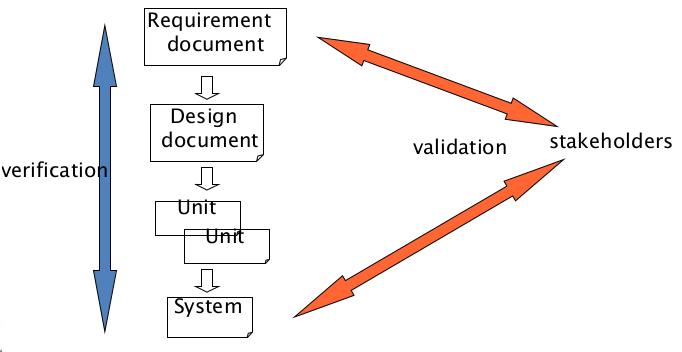
\includegraphics[scale=0.4]{images/v_v.png}
\caption{Verification and Validation}
\end{figure}

Cost of fixing defect increases incredibly during the software process from the requirement document to the complete system.

\begin{description}
\item [Failure] An execution event where the software behaves in an unexpected way. It is visible to the end user, who clearly knows that something is wrong.
\item [Fault] The feature of a software that causes a failure. May be due to an error in any part of the software, i.e.,\@ incomplete/incorrect requirements, test cases, database, etc.
\item [Defect] Generally speaking, a failure or a fault. A defect is characterized by an insertion activity and (hopefully) a removal activity. In fact, some defects may never be removed because they are minor or too much difficult to fix. It is needed to always assume that there are some defects and minimize the discovering time. The idea is to find as much defect as possible before software release.
\end{description}

Verification and validation is an horizontal activity because it happens during the entire duration of software. Basic goals of verification and validation are:
\begin{itemize}
\item Minimize number of defects inserted, it cannot be zero due to inherent complexity of software;
\item Maximize number of defects discovered and removed;
\item Minimize time span between insertion and discover and removal.
\end{itemize}

\begin{figure}[hbtp]
\centering
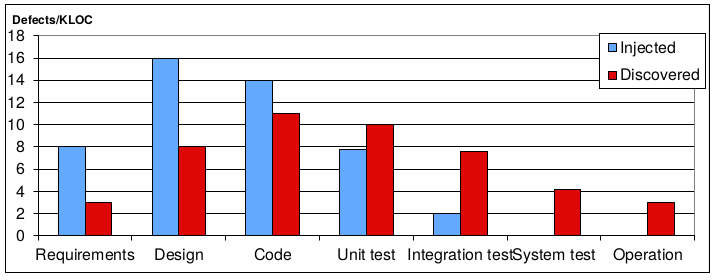
\includegraphics[scale=0.4]{images/defects_insertion_removal.png}
\caption{Insertion/removal by phase - Typical scenario}
\end{figure}

The longer the delay insert-remove, the higher the cost of removing defect. This is known as \textbf{rework problem}, shown in figure~\ref{img:rework_problem} where red color represents a perfect process, with a bell shape, while yellow color represents actual rework which is more similar to an exponential.

\begin{figure}[hbtp]
\centering
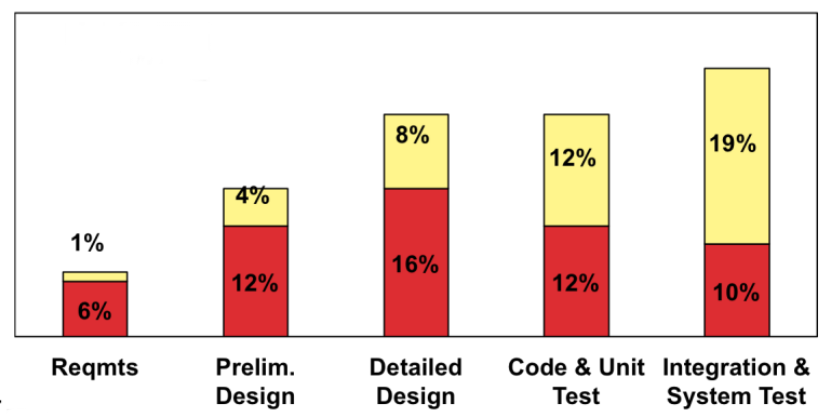
\includegraphics[scale=0.35]{images/rework_problem.png}
\caption{Rework problem}
\label{img:rework_problem}
\end{figure}

\section{Techniques}
\subsection{Static}
\subsubsection{Inspections}
\emph{Inspection} consist of reading documents and code by a group of people with goal of finding defects. Variants of inspections are reading techniques, walkthroughs or reviews. Many defects may be found, test phase concentrates one defect at a time.

\begin{figure}[hbtp]
\centering
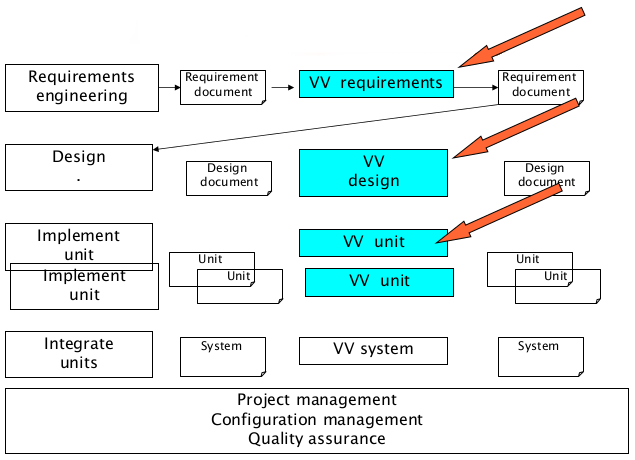
\includegraphics[scale=0.35]{images/v_v_inspection.png}
\caption{Inspection}
\label{img:v_v_inspection}
\end{figure}

This technique can be applied to documents and code. It is very effective because it reuses experience and knowledge of people on domain and technologies, therefore more global and dynamic groups can be used. However, it is more suitable for functional aspects and it requires time, i.e.,\@ effort and calendar time. Inspection and testing are complementary techniques and both should be used in V \& V.

Early defect detection improves product quality and reduces avoidable rework down to 10-20\%.

\paragraph{Roles in a group}
\begin{itemize}
\item \textbf{Moderator} leads inspection process and notably inspection meeting. It selects participants and prepares material. Usually, it is not from project that produces document to be inspected;
\item \textbf{Readers} read document to be inspected;
\item \textbf{Author} answers to questions that arise;
\item \textbf{Scribe} writes inspection log.
\end{itemize}

\paragraph{Fagan inspection process}
\begin{enumerate}
\item Planning: Select team, arrange materials, schedule dates;
\item Overview: Quickly present inspection group goals and document to be inspected;
\item Preparation: Important because inspectors are often unprepared. Read individually, applying inspection technique;
\item Inspection meeting: Team analysis to find defects. Group reads, discusses issues and agrees on problems. Scribe logs problems. Moderator keeps focus, keeps space and stops long discussions;
\item Rework: Author fixes defects/problem;
\item Follow-up: Repeat inspection or close and pass to next phase.
\end{enumerate}

Purpose of inspection is to find defects, not to fix them. Group aims to produce best possible document avoiding ``kill the author'' game and ``relax and chat'' meetings.

\subsubsection{Technique vs. document}
\paragraph{Defect taxonomies for requirements}
Identify categories of common defects.

\begin{Parallel}{0.45\textwidth}{0.45\textwidth}
\ParallelLText{
One level
\begin{itemize}
\item Omission;
\item Incorrect fact;
\item Inconsistency;
\item Ambiguity;
\item Extraneous information.
\end{itemize}
}
\ParallelRText{
Two levels
\begin{itemize}
\item Omission
\begin{itemize}
\item Missing functionality;
\item Missing performance;
\item Missing environment;
\item Missing interface.
\end{itemize}
\item Commission
\begin{itemize}
\item Ambiguous information;
\item Inconsistent information;
\item Incorrect fact or extra functionality;
\item Wrong section.
\end{itemize}
\end{itemize}
}
\end{Parallel}

\paragraph{Checklist for requirements}
Based on past defect information. Questions refine a defect taxonomy.

\paragraph{Checklist for code}
Dependent on programming language and on previous results of inspections.

\paragraph{Scenario-based reading}
Ask inspectors to create an appropriate abstraction which helps to understand the product. Ask inspectors to answer to a series of questions tailored to the abstraction. Inspectors follow different scenarios each focusing on specific issues.

\paragraph{Defect-based reading}
A scenario-based reading technique to detect defects in requirements expressed in a formal notation. Each scenario focuses on a specific class of defects (data type inconsistency, incorrect functionality, ambiguity or missing functionality).

\paragraph{Perspective-based scenario} Widespread technique. A scenario-based reading technique to detect defects in requirements expressed in natural language, extended later for design and source code. Each scenario focuses on reviewing the document from the point of view of a specific stakeholder.

For each requirement and functional specification, generate a test or set of tests that allow to ensure that an implementation of the system satisfies the requirements and functional specifications. During the reading, the reader has to produce something, helping the reader to be careful and to keep focused.

\subsection{Dynamic}
\subsubsection{Testing}
\emph{Testing} is a dynamic technique that requires execution of executable system or executable unit. The purpose of testing process is to find defects in the software products, which means that a test is successful if it reveals a defect. Indeed, it is easy to show that something works being very soft in its usage.

Testing is also the process of operating a system or component under specified conditions observing or recording the results to detect the differences between actual and required behavior.

Defect testing and debugging are different activities, which may be performed by different roles in different times. Testing tries to find failures, while debugging searches for and removes the fault. Debugging, actually, represents a short cycle of design and coding.

\begin{figure}[hbtp]
\centering
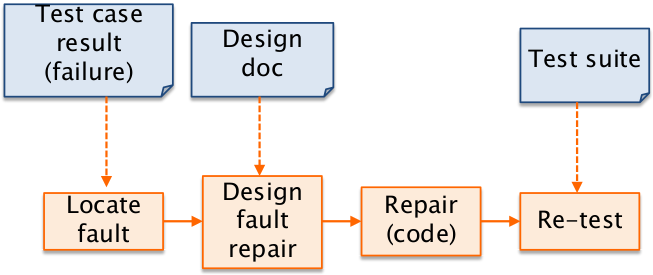
\includegraphics[scale=0.35]{images/debugging.png}
\caption{Debugging}
\end{figure}

\begin{description}
\item [Test case] Stimulus applied to executable, system or unit, composed by name, input and expected output with defined constraints and context, e.g.,\@ version and type of OS, DBMS, GUI, etc.
\item [Test suite] Set of related test cases. 
\item [Test case log] Composed by a test case reference, its time and date of application, its actual output and its result (passed or not passed).
\end{description}
Test activities:
\begin{enumerate}
\item Write test cases;
\item Run test cases (test suite);
\item Record results.
\end{enumerate}

\begin{figure}[hbtp]
\centering
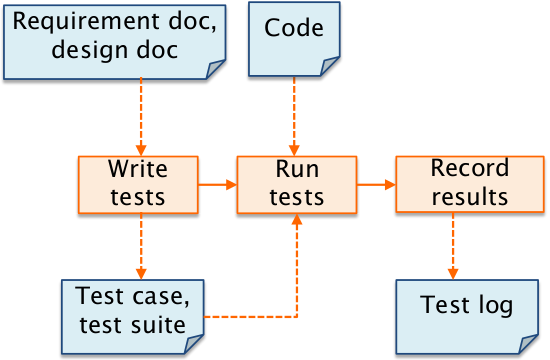
\includegraphics[scale=0.35]{images/test_activities.png}
\caption{Test activities}
\end{figure}

\paragraph{Possible scenarios}
\begin{enumerate}
\item Developer team and tester team are different. It is more complicated, longer and more expensive but it takes into account of different points of view, therefore more defects possibly arise;
\item Developer team both develops software and tests it. It is faster and cheaper but coverage is minor;
\item Developer team and tester team are different and after ``internal testing'', testing is repeated by a tester team (third party), possibly a certification authority, which ensures the quality. This approach is adopted in safety critical context.
\end{enumerate}

\paragraph{Oracle}
The ideal condition would be to have an automatic \emph{oracle}, very difficult to have, and an automatic comparator, available only is some cases. A human oracle is subject to errors. The oracle is based on the program specifications, which can be wrong. In order to perform testing, the expected behavior of a program for a given test case must be known.

A \emph{human oracle} is based on requirements specification or judgment.

An \emph{automatic oracle} is a model generated from formal required specification, e.g.,\@ the same software developed by other parties or previous version of program (possibly leading to regression).

\begin{figure}[hbtp]
\centering
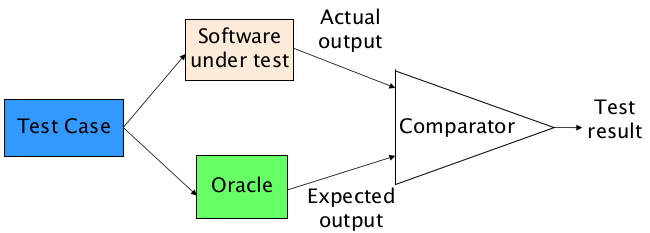
\includegraphics[scale=0.35]{images/oracle.png}
\caption{Oracle}
\end{figure}

\paragraph{Correctness}
\emph{Correctness}, in the sense of correct output for all possible input requires exhaustive testing, which is unfeasible. Thus, goal of test is to find defects (not demonstrating that system is defect free) and assure a \emph{good enough} level of confidence.

\subparagraph{Dijkstra thesis} Testing can only reveal the presence of error, never their absence.

\subparagraph{Weinberg's law} A developer is unsuitable to test his/her own code. Testing should be performed by a separate team or peers. If a developer misunderstand a problem, he cannot find any error.

\paragraph{Coverage} Test cases defined / Total test cases possible.

100\% and no failures $\Rightarrow$ correct.

\paragraph{Validity} A criterion is \emph{valid} if and only if, whenever the produced output is incorrect, such a criterion selects at least one test set which is not successful for the output.

\paragraph{Reliability} A criterion is \emph{reliable} if and only if, either every test selected by such a criterion is successful or no test selected is successful.

\subsection{Test classification}
\subsubsection{Testing per granularity level/phase}
\begin{itemize}
\item Unit tests: individual modules;
\item Integration tests: modules when working together;
\item System tests: the system as a whole usable system.
\end{itemize}

\begin{figure}[hbtp]
\centering
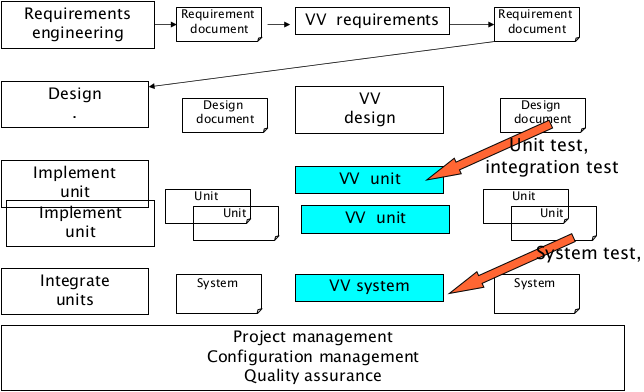
\includegraphics[scale=0.35]{images/testing_granularity_level.png}
\caption{Testing per granularity level/phase}
\end{figure}

\subsubsection{Testing per approach}
Given an object to test, approach can be:
\begin{itemize}
\item Requirements driven: are the requirements of the object satisfied?
\item Structure: is the object built as it should?
\item Reliability: does the object satisfy the customer need?
\item Risk: is the object vulnerable to most likely risks?
\end{itemize}

\begin{table}
\centering
\begin{tabular}{|c|c|c|c|}
\hline 
\multirow{2}{*}{} & \multicolumn{3}{c|}{\textbf{Phase}} \\ 
\cline{2-4}
 & \textbf{Unit} & \textbf{Integration} & \textbf{System} \\ 
\hline 
\textbf{Functional (Black box)} & • & • & • \\ 
\hline 
\textbf{Structural (White box)} & • &  & \\ 
\hline 
\textbf{Reliability} & & & • \\ 
\hline 
\textbf{Risks} & & & • \\ 
\hline 
\end{tabular}
\caption{Testing classification}
\end{table}

\begin{table}
\centering
\small
\begin{tabularx}{\textwidth}{|X|X|X|X|}
\hline 
 & \multicolumn{3}{c|}{\textbf{Testing phase}} \\ 
\hline
\textbf{Approach} & \textbf{Unit} & \textbf{Integration} & \textbf{System} \\ 
\hline 
\textbf{Requirements-driven} & 100\% unit requirements & 100\% product requirements & 100\% system requirements \\ 
\hline 
\textbf{Structure-driven} & 85\% logic paths & 100\% modules & 100\% components \\ 
\hline 
\textbf{Statistics-driven} & & & 90-100\% of usage profiles \\ 
\hline 
\textbf{Risk-driven} & As required & As required & As required \\ 
\hline 
\end{tabularx}
\caption{Testing classification and coverage}
\end{table}

\paragraph{Regression testing}
All tests used in the past must be performed and no more defects must be found in a newer version.

\section{Unit test}
\subsection{Black box}
\emph{Black box} testing is a functional test of units (functions, classes) which generates test cases starting from the specification of the unit. Source code is not needed.

\subsubsection{Random}
Random testing is independent of requirements but it requires many test cases. It is easy to define the inputs, but it requires an oracle to compute the expected output.

\subsubsection{Equivalence classes partitioning}
Input space is divided in partitions having similar behavior from the point of view of requirements for unit and a few test cases are performed for each partition. Boundary conditions must be defined to bound partitions and test cases are performed on the boundaries, too.

\paragraph{Equivalence class} A class corresponds to a set of valid or invalid inputs for a \emph{condition} on the input variables. If a test in a class has not success, the other tests in the same class should have the same behavior. Every equivalence class must be covered by a test case at least. Each test case for valid input classes must cover as many valid classes as possible.

\begin{enumerate}
\item Identify criteria, from requirements;
\item Define conditions for each criterion;
\item Define an order for combining conditions;
\item Combine conditions, identifying partitions;
\item Define one test case per partition.
\end{enumerate}

When a module has a state, the state has to be considered to define partitions. State may be difficult to read/create and it requires a sequence of calls. Typically, object oriented classes have state and many functions have to be tested. Criteria and equivalence classes have to be identified and applied to each function.

\subsection{White box}
\emph{White box} testing is structural and starts from the code, using several coverage objectives. White box testing is typically made in the development environment and supported by tools to compute coverage.

\paragraph{Statement coverage} Try to execute all statements in the program. \emph{Coverage} is a property of unit and test suite.
\[
\text{statement coverage} = \dfrac{\text{\# statements covered}}{\text{\# statements}}
\]
The main problem is the concept of statement. Programs can be transformed in \textbf{control flow graphs}. A node represents an atomic instruction, i.e.,\@ line terminated by a semicolon, or a decision, while an edge represents the transfer of control. Sequential nodes can be collapsed in a basic block. Statements which cannot be reached are called \emph{dead code}.

\emph{Control flow graph} makes more understandable which are the basic (atomic) statements.

\paragraph{Node coverage} Evaluated for each test, considered cumulative for a test suite.
\[
\text{node coverage} = \dfrac{\text{\# nodes executed}}{\text{\# nodes}}
\]

\paragraph{Decision coverage} Try to cover all decisions in the program. Also called edge coverage because a decision corresponds to an edge in the control flow graph.
\[
\text{decision coverage} = \dfrac{\text{\# decisions covered}}{\text{\# decisions}}
\]

\paragraph{Condition coverage}
\begin{itemize}
\item Simple condition coverage: each condition is at least once true and at least once false, but the final decision may be the same;
\item Multiple condition coverage: all the combinations must be tested. It may not be feasible in some cases.
\end{itemize}

\paragraph{Relationships}
\begin{gather*}
\text{Node coverage} \Leftrightarrow \text{Statement coverage} \\
\text{Basic block coverage} \Leftrightarrow \text{Statement coverage} \\
\text{Edge coverage} \Rightarrow \text{Node coverage} \\
\text{Edge coverage} \nLeftarrow \text{Node coverage} \\
\text{Multiple condition coverage} \Rightarrow \text{Decision coverage} \Rightarrow \text{Statement coverage} \\
\text{Multiple condition coverage} \Rightarrow \text{Simple condition coverage} \nRightarrow \text{Decision coverage}
\end{gather*}

\paragraph{Path coverage}
A \emph{path} is a sequence of nodes in a graph. Test cases should be selected in such a way that every path in the graph is visited. It may not be feasible, because of a combinatorial explosion with cycles. Some approximations are possible:
\begin{itemize}
\item Path-n: loop from 0 to n times in each loop;
\item Loop coverage: in each loop cycle 0, 1, > 1 times.
\end{itemize}

\paragraph{Loop coverage}
Test cases should be selected such that every loop boundary and interior is tested:
\begin{itemize}
\item Boundary: 0 iterations;
\item Interior: 1 iteration and > 1 iterations.
\end{itemize}
Consider each loop separately and write three test cases: no enter the loop, cycle once in the loop, cycle ore than once.

\paragraph{Test representation}
\begin{description}
\item [Informal] Using keyboard or screen. No documentation of test case, nor test log.
\item [Formal] Programming languages.
\end{description}
Tools are provided to write and run test cases (e.g.,\@ JUnit) and to compute coverage (e.g.,\@ Cobertura).

\subsection{Mutation testing}
\emph{Mutation testing} consists in evaluating the goodness of test cases. The basic idea is to inject errors in program with single small change and to verify if test cases catch the injected errors. This approach is used both in software and hardware.

\begin{description}
\item [Mutant] Program with one change.
\item [Killable mutant] Non functionally equivalent. A test case can kill it.
\item [Equivalent mutant] Functionally equivalent. No test case can kill it.
\item [Mutation score] Property of a test suite, goal is 100\%.
\[
\text{mutation score} = \dfrac{\text{\# kiled non equivalent mutants}}{\text{\# non equivalent mutant}}
\]
\end{description}

\paragraph{Common mutations}
\begin{itemize}
\item Delete a statement;
\item Swap two statements;
\item Replace arithmetic operations;
\item Replace boolean relations;
\item Replace a variable;
\item Replace boolean sub-expressions with constant value.
\end{itemize}
The main problem with mutation testing is time. In fact, many mutations are possible and a complete test suite is needed for each mutation.

\section{Integration testing}
Integration problems arise when more than one unit, possibly developed by different teams or in different time, interact together. In fact, it is possible that different conventions (i.e.,\@ parameters order, parameter names, unit of measurement, etc.) have been used, leading to unexpected results.

\begin{figure}[hbtp]
\centering
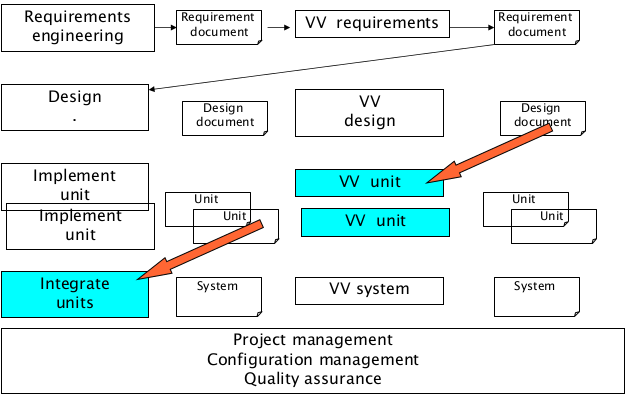
\includegraphics[scale=0.35]{images/integration_testing.png}
\caption{Integration testing}
\end{figure}

\paragraph{Dependency graph}
\emph{Dependency graph} shows dependencies among different units. It is useful to check if dependencies are correct.

\paragraph{Stub and driver}
A \emph{driver} is a unit (function or class) developed to pilot another unit. A \emph{stub} is a unit developed to substitute another unite, i.e.,\@ fake unit. They are also called \textbf{mock ups}.

A stub must be simpler with respect to the substituted unit, therefore it is needed to trade off simplicity and functionality, because a stub must be ``perfect'', i.e.,\@ without defects.

\subsection*{Big bang integration}
Test is applied directly to the aggregate as if it was a single unit. This approach does not focus on the dependencies, therefore it is difficult to locate a defect when it is found. A defect can be generated by any function or by any interaction.

\subsection*{Test units in isolation}
Each unit is tested independently by using stubs or driver. It may be possible that writing stubs is a difficult and costly operation, which must be taken into account.

\subsection*{Incremental integration}
Goal is to add one unit at a time and to test the partial aggregate. In this way, when a defect is found, most likely, it comes by last unit/interaction added, but more test cases, stubs and/or drivers have to be written.

\paragraph{Top down}
\emph{Top down integration} allows to early detect architectural flaws because a limited working system (prototype) is available early, but it is suitable only for top-down development, requires the definition of stubs for all lower level units which are not directly observable.

\paragraph{Bottom up}
\emph{Bottom up integration} can start early in the development process and lower levels are directly observable, but it requires the definition of drivers for all lower level units.

\subsection*{Hardware software integration}
\emph{Hardware software integration} is suitable for embedded systems. Usually writing stubs for sensors or actuators implies defining a simulated model of the context of the software application, as defined by context diagram and system design.

\begin{enumerate}
\item Test software units with stubs replacing hardware;
\item Integrate software and hardware.
\end{enumerate}

\section{System testing}
\emph{System testing} is applied to the software system as a whole. It aims at verifying the correspondence of the system to the requirements. Typically it is not performed by the development team, but by a test team. Functional requirements are tested by covering use cases as listed in the requirement document and considering usage profile, i.e.,\@ typical ways of using the system. Test is performed in conditions close, as far as possible, to the working ones.

\begin{figure}[hbtp]
\centering
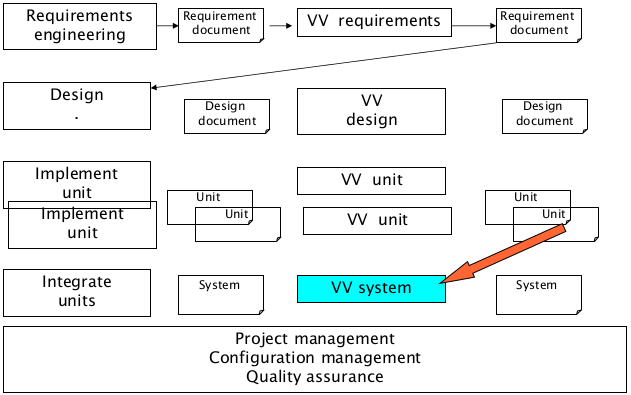
\includegraphics[scale=0.35]{images/system_testing.png}
\caption{System testing}
\end{figure}

\paragraph{Platform} The \emph{platform} is the environment where an application runs, defined by operating system, database, network, memory, CPU, libraries, etc.

An element can be tested on:
\begin{itemize}
\item \textbf{Target platform}: where the element will run for day by day use. It cannot be used for production because data may be corrupted and it may not be available;
\item \textbf{Production platform}: where the element is produced. It cannot be, in most cases, equal to the target platform.
\end{itemize}
For an embedded system, production platform is typically a PC, with simulated/emulated external devices, while for an information system, is typically a PC or a workstation, with a replicated database in a simplified form.

\paragraph{Variants}
System testing can be performed by end user (beta testing) or developer on development or target platform. \emph{Acceptance testing} is made by the user, possibly on both development and target platforms. Typically, it considers data and test cases provided by the customer on target platform.

\medskip

System testing tests non functional requirements, which are usually emerging properties, in many cases testable only when the entire system is available, e.g.,\@ efficiency, reliability.

\paragraph{Non functional properties}
\begin{itemize}
\item Configuration: the commands and mechanisms to change the system;
\item Recovery: the capability of the system to react to catastrophic events;
\item Stress: reliability of the system under limit conditions, e.g.,\@ huge number of users;
\item Security: resilience to non authorized accesses.
\end{itemize}

\begin{table}
\centering
\begin{tabular}{|c|c|c|c|}
\hline 
 & \multicolumn{3}{c|}{Phase} \\ 
\cline{2-4} 
 & Unit & Integration & System \\ 
\hline 
Functional (Black box) & • & • & • \\ 
\hline 
Structural (white box) & • & & \\ 
\hline 
Reliability & & & • \\ 
\hline 
Risks & & & • \\ 
\hline 
\end{tabular} 
\caption{Testing classification}
\end{table}

\paragraph{Reliability testing}
\emph{Reliability testing} aims at providing estimation of reliability, i.e.,\@ probability of failure over a period of time. Other possible measures are $\text{defect rate} = \text{defect}/\text{time}$ or $\text{MTBF} = \text{time between defects}$. In order to estimate reliability, a large number of independent test cases are needed, and defect fix must not introduce other defect, i.e.,\@ regression testing.

\begin{figure}[hbtp]
\centering
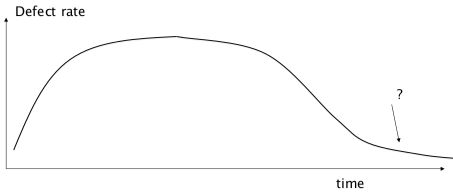
\includegraphics[scale=0.4]{images/software_reliability.png}
\caption{Software reliability}
\end{figure}

\paragraph{Risk based testing}
\begin{enumerate}
\item Identify risks;
\item Characterize risks: probability, effect;
\item Rank risks;
\item Handle risks.
\end{enumerate}

\paragraph{User profile based testing}
\emph{User profile based testing} is a variant of risk based testing:
\begin{enumerate}
\item Identify user profiles and usage profiles;
\item Rank them by frequency of usage;
\item Test more more used profiles.
\end{enumerate}
This approach is typically adopted on widespread software, e.g.,\@ MS Word.

\paragraph{Regression testing}
Tests previously defined are repeated after a change to assure that the change has not introduced defects. In general, it is applied to all objects, i.e.,\@ unit tests, integration tests and acceptance tests.

\begin{table}
\centering
\small
\begin{tabularx}{0.95 \textwidth}{|X|X|X|X|X|}
\hline 
 & Functional / Non functional & Who tests & Platform & Techniques \\ 
\hline
\textbf{Unit test} & Functional / Structural & Developer or test group & Production  & BB, WB\\ 
\hline 
\textbf{Integration test} & Functional & Developer or test group & Production & Incremental\footnote{Also called grey box, i.e.,\@ internal testing but not so internal as white box.} TD or BU\\ 
\hline 
\textbf{System test} & Functional + Non functional & Developer or test group or user & Production, target & Requirement coverage, use case coverage \\ 
\hline 
\end{tabularx}
\caption{Testing}
\end{table}

\section{Documentation and automation}
%Non documenting test cases is a possible technique to perform informal and exploratory testing. 
Representing test cases can be done:
\begin{itemize}
\item Informally: reading is easy, but test cases are not executable, e.g.,\@ Word document;
\item Formally:
\begin{itemize}
\item Word/Excel document and translator to programming language, e.g.,\@ FIT, Fitness;
\item Programming language: executable and easily reusable (i.e.,\@ regression testing) but less readable, e.g.,\@ Eclipse + JUnit or similar.
\end{itemize}
\end{itemize}
Test cases should be documented, so that they are not lost and can be reapplied and automated, so that application of test cases is fast and error free.

\subsection{Testing tools}
\paragraph{Table based testing}
Test cases are written as tables in Word or Excel, and linked to application ones the to be tested. In this way, end users are allowed to write tests, especially acceptance and black box ones, tests are independent of GUI and automation is possible. \emph{Fixtures} are needed to translate input from the table to the input of a coded function, to compare expected result to the actual one and to write the result. Using this approach, checking complex scenarios is difficult.

\paragraph{FIT framework for integrated testing}
Open source implementation of table based testing. User specifies tests in HTML tables, developer defines fixtures to parse tables and executes tests, while FIT compares tables and actual results. \emph{FITnesse} is a standalone wiki allowing group to easily edit test files without worrying about ensuring the correct versions are propagated out to all locations.

\paragraph{Coverage}
Show graphically and numerically coverage on source code, e.g.,\@ Cobertura, Eclemma.

\paragraph{Profilers}
Trace time spent per function, given specific test executions, i.e.,\@ performance test.

\subsubsection{GUI testing tools}
GUI testing is the practice of testing a GUI software through its user interface.
\begin{itemize}
\item \textbf{Functional testing}: black box tests exercising the basic functionalities of an application through interaction with the GUI, without knowing the source code;
\item \textbf{Look \& feel verification}: GUI should appear as defined in the requirements document, or in the mockups provided by the stakeholders.
\item \textbf{Compatibility testing}: testing that the application is deployed and behaving properly on different devices, screens and layouts (device diversity).
\end{itemize}

\paragraph{Approaches}
\begin{description}
\item [Manual] Manual execution of test scenarios.
\begin{itemize}
\item Easy to setup, not tools required;
\item Error prone, hardly reproducible, expensive.
\end{itemize}
\item [Scripted] Development of test scripts using dedicated scripting languages.
\begin{itemize}
\item Scripts can be automatically executed and used for regression testing;
\item Test scripts can be difficult to write and hard to maintain during the evolution of the software.
\end{itemize}
\item [Capture \& replay] User inputs are given once to the user interface (CAPTURE) and then codified into a repeatable script (REPLAY).
\begin{itemize}
\item Faster and easier to obtain test scripts with respect to pure scripted techniques;
\item Very fragile to the evolution of the user interface;
\item Script must be enriched manually to perform complex operations.
\end{itemize}
\item [Model-based] Test cases are obtained based on models of the user interface (e.g.,\@ oriented graphs or finite state machines).
\begin{itemize}
\item Allow automated execution and generation of use cases;
\item Very high coverage of use cases and functionalities can be obtainable once a model is available;
\item Manual effort required in defining and tailoring the GUI model.
\end{itemize}
\item [Visual testing] Image recognition techniques are used to identify elements of the user interface to interact with.
\begin{itemize}
\item Easy definition of test cases with no need of technical knowledge - only screen captures are needed;
\item Can be applied seamlessly to any kind of software provided with an (emulated) user interface;
\item Very high fragility to even minor changes in the GUI;
\item Difficult in-depth testing of application functionalities.
\end{itemize}
\end{description}

\subsection{Test documentation}
\emph{IEEE Standard for Software Test Documentation} defines the deliverables to be produced by the testing process avoiding duplication between documents and between documents and tools.

\begin{figure}[hbtp]
\centering
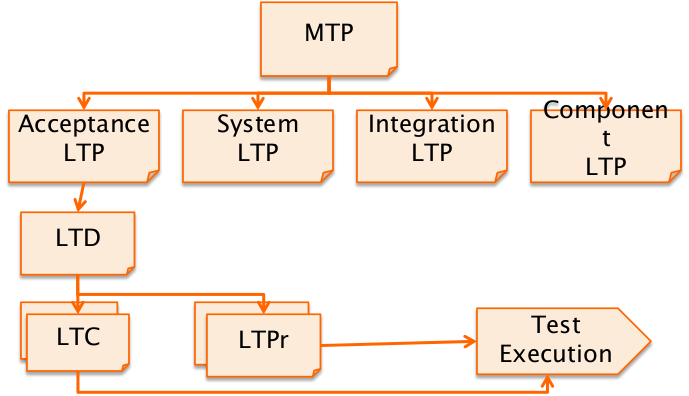
\includegraphics[scale=0.3]{images/deliverables.png}
\caption{Relationship among deliverables}
\end{figure}

\subsubsection{Planning and specification documents}
\paragraph{Master test plan}
\emph{Master test plan} guides the management of testing, establishes a plan and schedule, defines the required resources and generic pass/fail criteria, identifies the test items and explains the nature and extent of each test.

\paragraph{Level test plan}
\emph{Level test plan} defines testing activities (scope, approach, resources and schedule) and identifies items being tested, features to be tested, testing tasks to be performed, personnel responsible for each task and associated risks.

\paragraph{Traceability matrix}
\emph{Traceability matrix} maps tests to requirements and identifies which tests passed, and hence which requirements are satisfied. It may be part of the test plan.

\paragraph{Test design specification}
\emph{Test design specification} specifies, for one or more features to be tested, the details of the approach, i.e.,\@ testing techniques, analysis of results, list of test cases and motivation, generic attributes.

\paragraph{Test case specification}
\emph{Test case specification} specifies a test case in terms of goal, input data, expected output (oracle), test conditions (required hardware and software), special procedural requirements and inter-test dependencies. The test case is listed in a TDS document.

\paragraph{Test procedure specification}
\emph{Test procedure specification} specifies how to execute one or more test cases. The test procedure defines how to prepare the execution of the test, how to start and conduct the execution, which measurement to collect, how to suspend the test in presence of unforeseen events and how to resume a suspended test.

\subsubsection{Enactment documents}
\paragraph{Execution deliverables}
Test item transmittal report which must describe a test item delivered for test and include at least identification of software item, its status and physical location. Test log, which must be a complete, systematic and chronological report of all details relative to test execution.

\begin{figure}[hbtp]
\centering
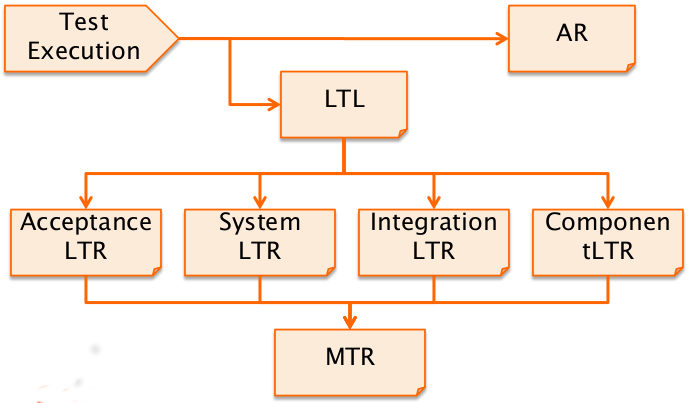
\includegraphics[scale=0.3]{images/deliverables_execution.png}
\caption{Execution deliverables}
\end{figure}

\paragraph{Level test log}
\emph{Level test log} provides a chronological record of relevant details about test execution. An automated tool may capture all or part of this information. It must include relevant info, i.e.,\@ execution description, procedure results, environment and anomalies.

\paragraph{Anomaly report}
\emph{Anomaly report} documents any event that occurred during the testing process that requires investigation, including information about its time, its context, its impact and a description of input, expected and actual output and anomalies.

\paragraph{Interim test status report}
\emph{Interim test status report} summarizes the results of testing activities, including test status summary, changes from plans and test status metrics.

\paragraph{Level test report}
\emph{Level test report} summarizes the results of designated testing activities, including an overview of results, detailed results, i.e.,\@ open and resolved anomalies, test executed and collected metrics and test assessment, and recommendations, i.e.,\@ test items evaluation and suitability for production use.

\paragraph{Master test report}
\emph{Master test report} summarizes the results of all testing activities, including test tasks results, list of anomalies and resolutions, assessment of release quality and summary of collected metrics.

\section{Static analysis techniques}
These techniques are applied directly to the source code. Code is read by some tools without its execution.

\subsection{Compilation analysis}
Compilers analyze the code checking for syntax, types and semantic correctness. The errors detected by a compiler strongly depend on the language, e.g.,\@ loose or strongly typed.

\paragraph{MISRA-C}
\emph{Motor Industry Software Reliability Association} defines guidelines for C in order to limit possible but dangerous operations. For example:
\begin{itemize}
\item Use only character in the source character set. This excludes the characters \texttt{\$} and \texttt{@}, among others;
\item Declarations of identifiers denoting objects should the narrowest block scope unless a wider scope is necessary;
\item The operands of the \texttt{\&\&} and \texttt{||} operators shall be enclosed in parenthesis unless they are single identifiers;
\item Identifiers modified within the increment expression of a loop header shall not be modified inside the block controlled by that loop header;
\item Relational operators shall not be applied to objects of pointer type except where both operands are of the same type and both point into the same object.
\end{itemize}
Each rule should help to have a more reliable software. Source code is parsed, checking if rules are violated.

\paragraph{Bad smells}
Some indicators are specified to possibly detect issues. Mostly, these are design issues not strictly related to the code and they are not automatically recognizable by a tool, hence they have to be manually checked.

\begin{multicols}{2}
\begin{itemize}
\item Duplicated code;
\item Long method;
\item Large class;
\item Long parameter list;
\item Lazy class;
\item Message chain;
\item Middle man;
\item Incomplete library class.
\end{itemize}
\end{multicols}

\subsection{Data flow analysis}
\emph{Data flow analysis} analyzes the values of variables during execution to find out anomalies. It looks like dynamic but some information can be collected statically.
\begin{itemize}
\item Definition (write): a new value is assigned;
\item Use (read): the value of the variable is read;
\item Nullification: the variable has no significant value;
\end{itemize}
This approach is unfeasible in ``complicated'' code containing if-then-else or loop statements.

A \emph{correct sequence} is the one where the use of a variable is preceded by a definition of the same variable. A \emph{suspect/forbidden sequence} is the one where the use of a variable is not preceded by a definition. In fact, this corresponds to the use of an undefined value.

Some tools recover the sequence and recognize suspect ones.

\paragraph{Symbolic execution}
The program is executed with symbolic values instead of actual values. Output variables are expressed as symbolic formulas of input variables. Symbolic execution may be extremely complex even for simple programs.

\section{Certifications}
ISQTB (\href{www.isqtb.org}{www.isqtb.org}) is the International Software Testing Qualifications on Board, with delegations in most countries. It publishes Syllabus, which are available for free and provides certifications, via exams at different levels: foundation, advanced and expert on core, agile and specialist tracks.